\chapter{CORRECTION OF ERRORS}
\subsection{Sources of Error in Cryptography}

Errors, mutilations, and garbles are some of the names applied to the
inaccuracies that occur in cryptographic communication. They are so
common and so troublesome that commanders who, for the most part,
already regard cryptographic processes as hopelessly slow and cumbersome, often become much prejudiced against their use in active opera-
tions. Therefore, instruction in the correction of errors is an essential
part of the training of personnel assigned to cryptographic work. Train—
ing and experience will reduce the time necessary to correct the most
common types of errors, which may be traced to the following sources:
\begin{enumerate}[label=\alph*]
\item Cryptographing and decryptographing, including the simple process
of copying by hand or by typewriter.

\item Transmission and reception by all means of signal communication
other than those in which the cryptograms are physically carried from
origin to destination.
\end{enumerate}

\subsection{Practical Suggestions for Eliminating Errors}

\mypara Errors in cryptographing and decryptographing can be much
reduced though not wholly eliminated, by systematizing the work so far
as possible and invariably checking it. Great care must be exercised in
the formation of letters in writing, and roman capitals should always be
used. If copied messages are checked for correctness by two operators,
one reading the letters to the other, a phonetic alphabet must be used in
order to prevent misunderstandings. In forward areas it is impossible to
provide suitable or convenient quarters for personnel engaged in cryptographic work, but in rear areas and at the larger headquarters this per-
sonnel will work much more efficiently in a quiet, well ventilated office.
To check the accuracy of cryptographic work it is always advisable, when
possible, that an operator other than the original cryptographic clerk
decryptograph the message. In checking his own work, an operator should
actually decryptograph it—not merely check his cryptographing—because
it is a psychological fact that persons have a tendency to repeat an error
unconsciously. The most serious errors in cryptographic work leading to
difficulties and delays in decryptographing are not the mere mistakes in
the writing down of letters, but are errors of a fundamental nature which
the operator says, when it comes back to him, “I don’t see how I could
have made it.” Checking by actually decryptographing will usually elimi-
nate such errors. At the destination, the final copy of a decryptographed
message should invariably be checked against the original work sheets
before being turned over to the addressee, and again preferably, by
another operator. It is easy to omit the word NOT from a decoded
message and to fail to note the omission, if the same operator merely
reads over the decryptographed message. Here, again, psychological
factors are involved, and clerks who are disposed to transpose letters and
words, an unconscious habit of a peculiar psychological origin, must be
especially careful in their work.

\mypara Carelessness in the writing of system and message indicators, or
failure to insert them in their proper places in the message, will usually
make prompt decryptographing of the received message difficult or
impossible. They should be written with the greatest of care.

\mypara If an incoming message is partially or wholly unreadable, an attempt
should be made to find the error in the faulty message. Often a message
can be decryptographed by a simple expedient such as applying the key
for the day preceding or following and correct date, or applying the daily
key for a classification higher or lower and the correct classification. If,
however, the garbled text still resists all efforts of correction, a procedure
(service) message should be sent. The length of time one should con-
tinue with the attempt to break the faulty message before sending a
service will depend upon the classification and precedence of the message,
transmission problems involved, time required to complete service, etc.

\mypara The procedure in preparing and handling service messages dealing
with errors in cryptographic messages is quite involved, in order not to
compromise the cryptographic system or give clues as to the contents of
the faulty message. Instructions covering the procedure to be followed
in such Servicing are issued from time to time and should be carefully
followed.

\mypara The most important precaution to be observed, in order to avoid the
transmission-of messages which cannot be promptly decryptographed at
the receiving end, is the rigid adherence to all instructions set forth in
documents describing the cryptographic operations to be followed. Misunderstanding or ambiguity is rarely found in properly prepared docu-
ments detailing cryptographic operations, and a careful study and
observance of the instructions will result in the preparation of messages
without fundamental errors.

\mypara To be efficient in cryptographic work requires, in addition to the
usual qualities -of carefulness, accuracy, and attention to detail, the
possession of certain psychological characteristics peculiar to the work. If
absent, these characteristics as a rule cannot be developed, but if present
they can be intensified and made more efficient by constant practice and
experience. It is therefore advisable to select personnel for cryptographic
work as for any other specialized work, to train them carefully, and
retain them as long as possible; the longer they remain in this work the
less likely they are to repeat the errors with which the work abounds and
:the more likely they are to render highly efficient service.

\mypara Errors in transmission and reception are frequently made, especially
in transmission by radio, because of interference, atmospheric disturb:ances, and the like. Cryptographic clerks should be familiar with the
Morse and Bandot alphabets and the most common errors of wire and
:radio transmission methods, so as to be able to refer an error to its
probable origin or to find clues for the correction of badly garbled groups
\when all other means fail. The following tables will be found useful:

\begin{figure}[h]
   \centering
    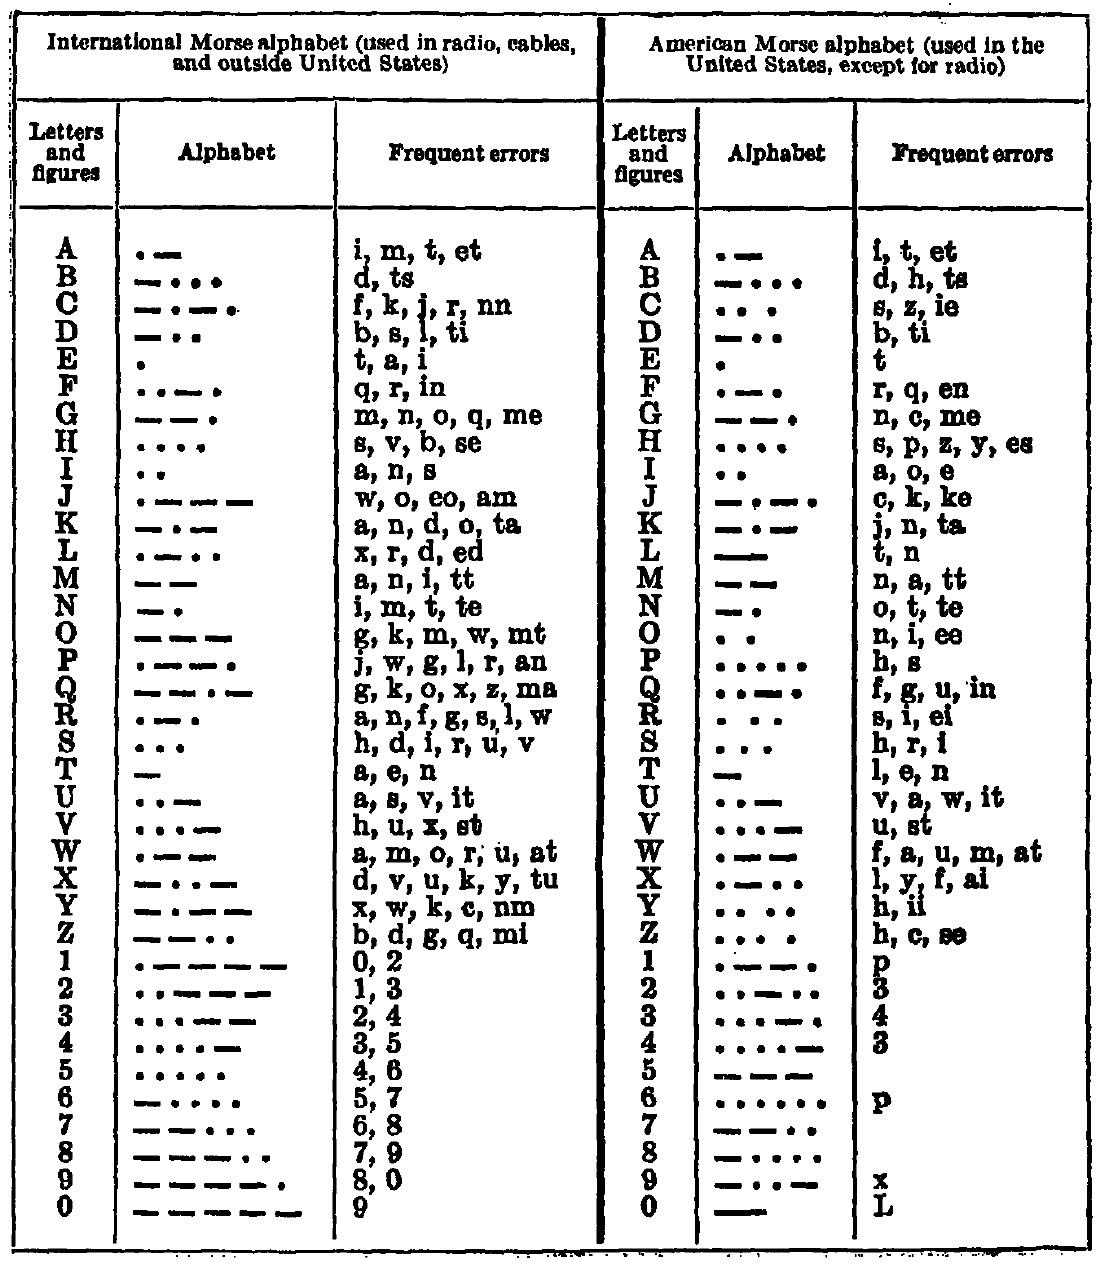
\includegraphics[width=0.9\textwidth,natwidth=1111,natheight=1275]{Chapter6_Figure1.eps}
\end{figure}


\begin{figure}[h]
   \centering
    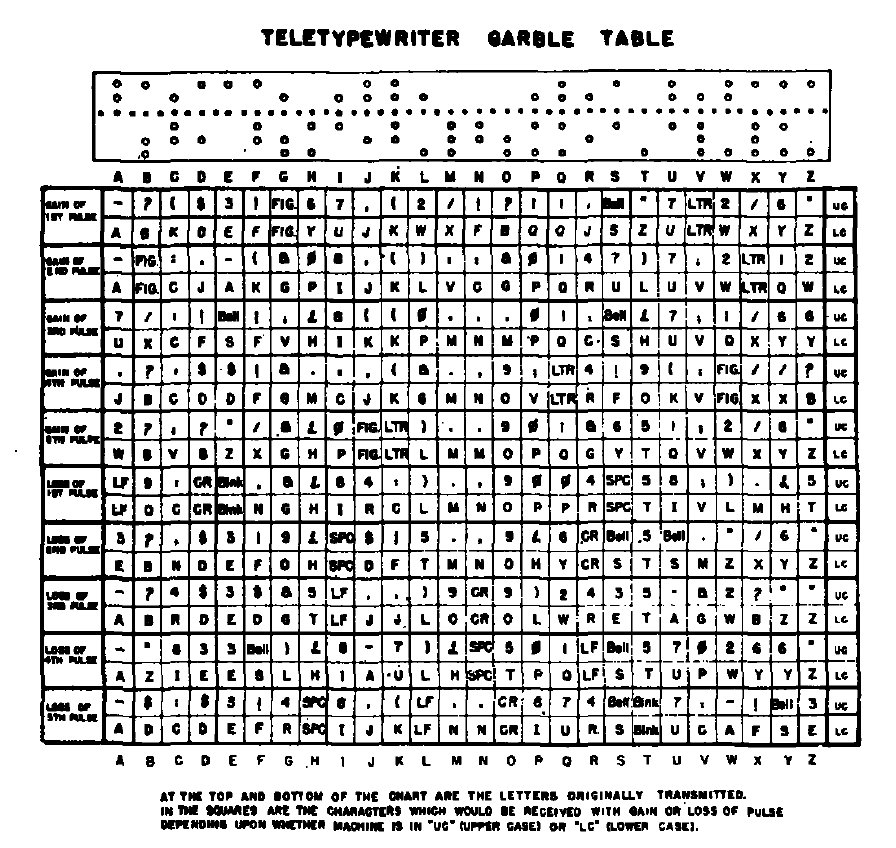
\includegraphics[width=1.0\textwidth,natwidth=896,natheight=848]{Chapter6_Figure2.eps}
\end{figure}
